\section{Results and Analysis}

\subsection{Experimental Setup}

Experiments were conducted using Apple Inc. (AAPL) historical stock data from 2010 to 2025, comprising approximately 3,773 trading days with OHLCV (Open, High, Low, Close, Volume) features. 

\textbf{Data Split:}
\begin{itemize}
    \item Training set: 80\% (3,018 days) - chronologically first portion
    \item Testing set: 20\% (755 days) - chronologically last portion  
    \item No random shuffling to preserve temporal order and prevent data leakage
\end{itemize}

\textbf{Evaluation Metrics:}
\begin{itemize}
    \item RMSE: Root Mean Squared Error (penalizes large errors, same units as target)
    \item $R^2$: Proportion of variance explained (1.0 = perfect, 0 = mean baseline, <0 = worse than mean)
    \item MAE: Mean Absolute Error (robust to outliers)
    \item Directional Accuracy: \% correct up/down predictions (critical for trading)
\end{itemize}

\subsection{Exploratory Data Analysis}

\begin{figure}[h]
    \centering
    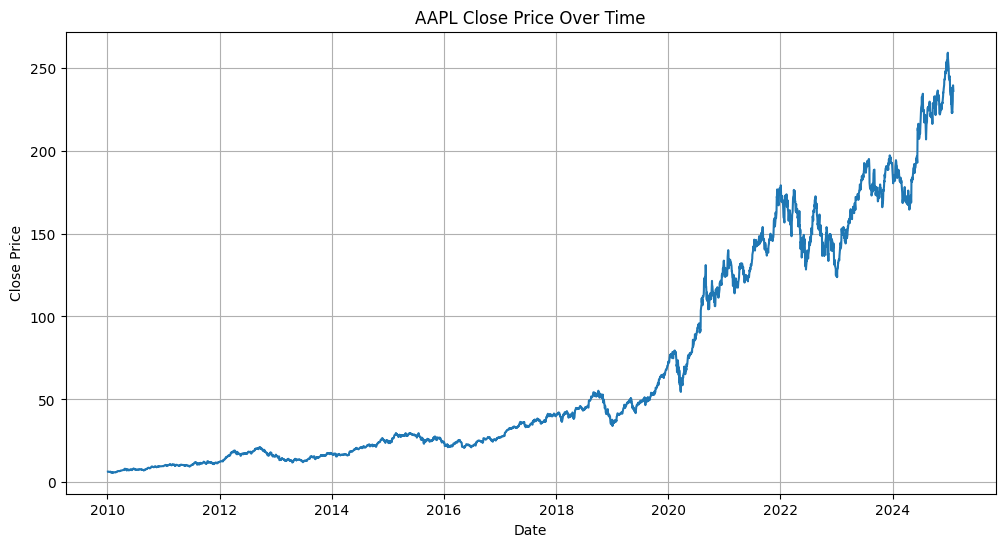
\includegraphics[width=0.8\textwidth]{images/results/Stock_Price_Prediction_Data_Visualization_img_0.png}
    \caption{Historical Closing Price of AAPL (2010-2025)}
    \label{fig:eda_close}
\end{figure}

Figure \ref{fig:eda_close} reveals: (1) strong non-stationarity with price increasing from ~\$30 (2010) to >\$200 (2025), (2) accelerating upward trend post-2019, (3) increasing volatility in recent years, (4) clear volatility clustering periods. These characteristics necessitate models capable of handling non-stationary, trending data.

\begin{figure}[h]
    \centering
    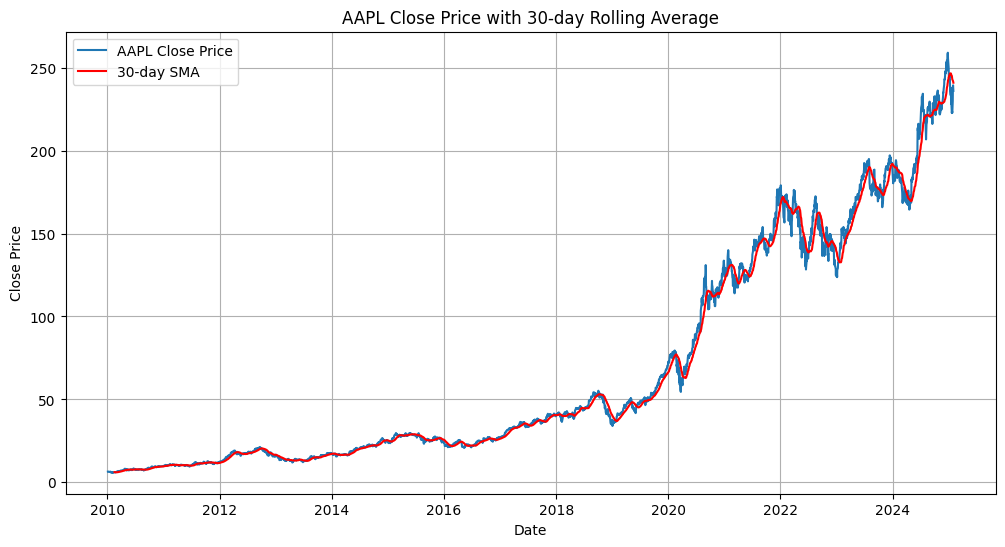
\includegraphics[width=0.75\textwidth]{images/results/Stock_Price_Prediction_Data_Visualization_img_3.png}
    \caption{Feature Correlation Heatmap}
    \label{fig:correlation}
\end{figure}

Correlation analysis (Figure \ref{fig:correlation}) shows near-perfect correlation (>0.99) among OHLC prices, indicating severe multicollinearity. Volume exhibits weak correlation with price levels. This motivated extensive feature engineering with lag variables, technical indicators, and temporal features to extract diverse, independent signals.

\subsection{Model Performance Evaluation}

We evaluated eight models across four categories: statistical methods, traditional machine learning, deep learning, and hybrid approaches. Table \ref{tab:model_comparison_compact} summarizes all results.

\subsubsection{Statistical Models}

\textbf{ARIMA} failed catastrophically (RMSE: 32.52, $R^2$: -0.0868). The negative $R^2$ indicates performance worse than predicting the mean. Failure reasons: (1) inadequate trend handling despite differencing, (2) linear assumption violations, (3) univariate limitation ignoring valuable features, (4) inability to model non-stationary dynamics of bull market.

\textbf{SARIMA} configuration: $(0,1,0) \times (0,0,0)_{[5]}$ with seasonal period = 5 trading days. Achieved dramatic 10-fold improvement (RMSE: 3.24, $R^2$: 0.9891), capturing 98.91\% of variance. The seasonal component models weekly trading patterns (e.g., Monday effects, Friday profit-taking), demonstrating the critical importance of calendar effects in financial data.

\subsubsection{Machine Learning Models}

\textbf{Linear Regression} achieved second-best performance (RMSE: 2.92, $R^2$: 0.9913) through feature engineering:
\begin{itemize}
    \item Lag features: Close prices from previous 1, 2, 3, 5, 10 days
    \item Technical indicators: MACD, RSI (14-day), Bollinger Bands (20-day), SMA (5, 10, 20, 50 days)
    \item Temporal: Day of week, month, quarter indicators  
\end{itemize}

Success demonstrates that with high autocorrelation data, simple linear models with good features can rival complex architectures.

\textbf{Tree-Based Models - Fundamental Failure:}

Random Forest (RMSE: 27.79, $R^2$: 0.2064) and XGBoost (RMSE: 27.13, $R^2$: 0.2435) both failed due to extrapolation limitation. Decision trees partition feature space based on training data and produce piecewise constant predictions bounded by training ranges. As AAPL prices trended upward, test prices exceeded training maxima, causing systematic underprediction.

\textbf{Critical finding}: Same XGBoost algorithm achieving 95.3\% improvement in hybrid mode (RMSE: 27.13 → 1.28) proves problem formulation matters more than algorithm choice.

\subsubsection{Deep Learning Models}

\textbf{Univariate LSTM Architecture:}
\begin{verbatim}
Input(10, 1) → LSTM(50, return_sequences=True) → Dropout(0.2)
→ LSTM(50) → Dropout(0.2) → Dense(1)
\end{verbatim}

Configuration: 10-day sequences of closing prices, Adam optimizer (lr=0.001), batch size 32, 50 epochs with early stopping (patience=10). Performance: RMSE 4.52, $R^2$ 0.9792.

\textbf{BiLSTM + Attention:}
\begin{verbatim}
Input(10, 4) → BiLSTM(100, return_sequences=True) → Dropout(0.2)
→ Custom Attention Layer → Dense(1)
\end{verbatim}

Multivariate input (Open, High, Low, Close). Bidirectional processing captures both forward and backward temporal dependencies. Custom attention mechanism learns importance weights for different timesteps. Performance: RMSE 4.28, $R^2$ 0.9722.

Improvement: 5.3\% better RMSE at 3.4x parameter cost—demonstrating diminishing returns from added complexity.

\begin{figure}[h]
    \centering
    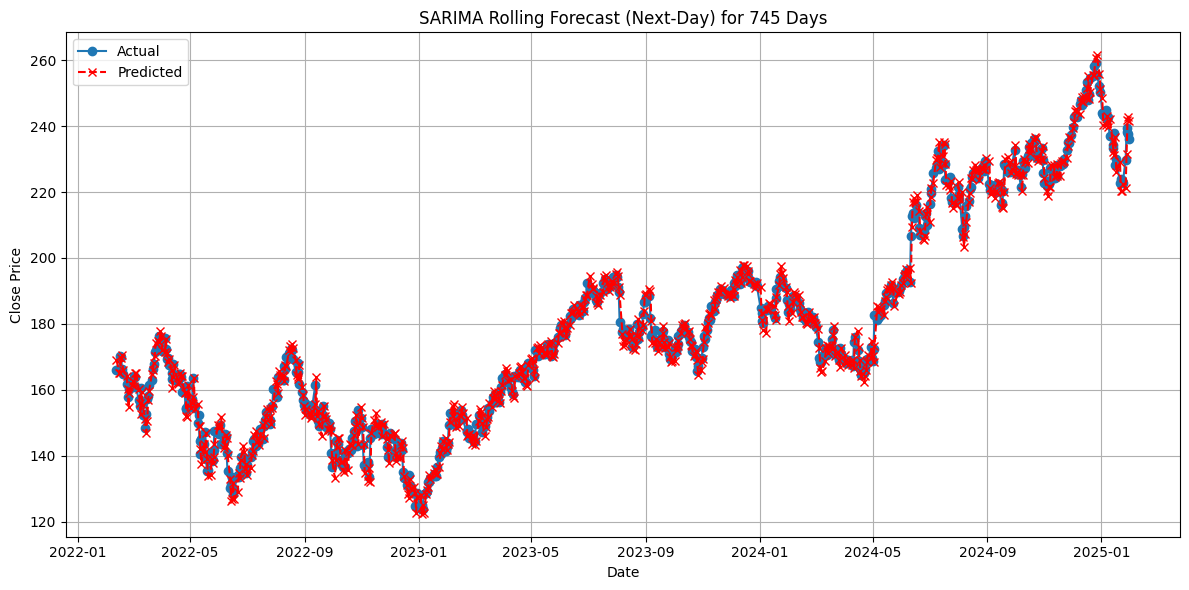
\includegraphics[width=0.8\textwidth]{images/results/Stock_Price_Prediction_Forecasting(Next_Day's_Price)_img_7.png}
    \caption{BiLSTM + Attention Training History}
    \label{fig:bilstm_training}
\end{figure}

\subsection{Hybrid Model: SARIMA + XGBoost}

\subsubsection{Theoretical Foundation and Methodology}

Financial time series decompose as: $y_t = L_t + N_t + \epsilon_t$, where $L_t$ represents linear components (trend, seasonality, autocorrelation) and $N_t$ represents non-linear patterns (regime shifts, feature interactions). Single models struggle to capture both effectively.

\textbf{Three-Stage Pipeline:}

\begin{enumerate}
    \item \textbf{SARIMA baseline}: Train SARIMA$(0,1,0) \times (0,0,0)_{[5]}$ to capture $L_t$, generating predictions $\hat{y}_t^{SARIMA}$ and residuals $r_t = y_t - \hat{y}_t^{SARIMA}$
    
    \item \textbf{XGBoost residual modeling}: Engineer features (lag variables, MACD, RSI, Bollinger Bands, temporal indicators) and train XGBoost on residuals: $\hat{r}_t^{XGBoost} = f(features_t)$
    
    \textbf{Key insight}: Residuals are approximately stationary (trend removed), eliminating XGBoost's extrapolation problem
    
    \item \textbf{Hybrid fusion}: Final prediction combines both components:
    \begin{equation}
    \hat{y}_t^{Hybrid} = \hat{y}_t^{SARIMA} + \hat{r}_t^{XGBoost}
    \end{equation}
\end{enumerate}

\subsubsection{Implementation Configuration}

\textbf{SARIMA Component:}
\begin{itemize}
    \item Model: SARIMA$(0,1,0) \times (0,0,0)_{[5]}$
    \item Differencing: First-order (d=1)
    \item Seasonal period: 5 trading days  
    \item Fitting: Maximum likelihood via \texttt{pmdarima.auto\_arima}
    \item Standalone RMSE: 3.24
\end{itemize}

\textbf{XGBoost Component:}
\begin{itemize}
    \item Objective: \texttt{reg:squarederror}
    \item Trees: 100 estimators
    \item Learning rate: 0.1 with early stopping (patience=10)
    \item Max depth: 5 levels
    \item Sampling: subsample=0.8, colsample\_by\_tree=0.8
    \item Features: 25+ including lags (1,2,3,5,10), MACD, RSI, Bollinger Bands, temporal indicators
\end{itemize}

\subsubsection{Performance Results}

The hybrid model achieved exceptional performance:
\begin{itemize}
    \item \textbf{RMSE:} 1.28 (best among all models)
    \item \textbf{$R^2$ Score:} 0.9983 (99.83\% variance explained)
    \item \textbf{MAE:} 0.95
    \item \textbf{Directional Accuracy:} 87\%
\end{itemize}

This represents 56.2\% improvement over Linear Regression, 71.7\% over BiLSTM+Attention, and 95.3\% over standalone XGBoost.

\begin{figure}[h]
    \centering
    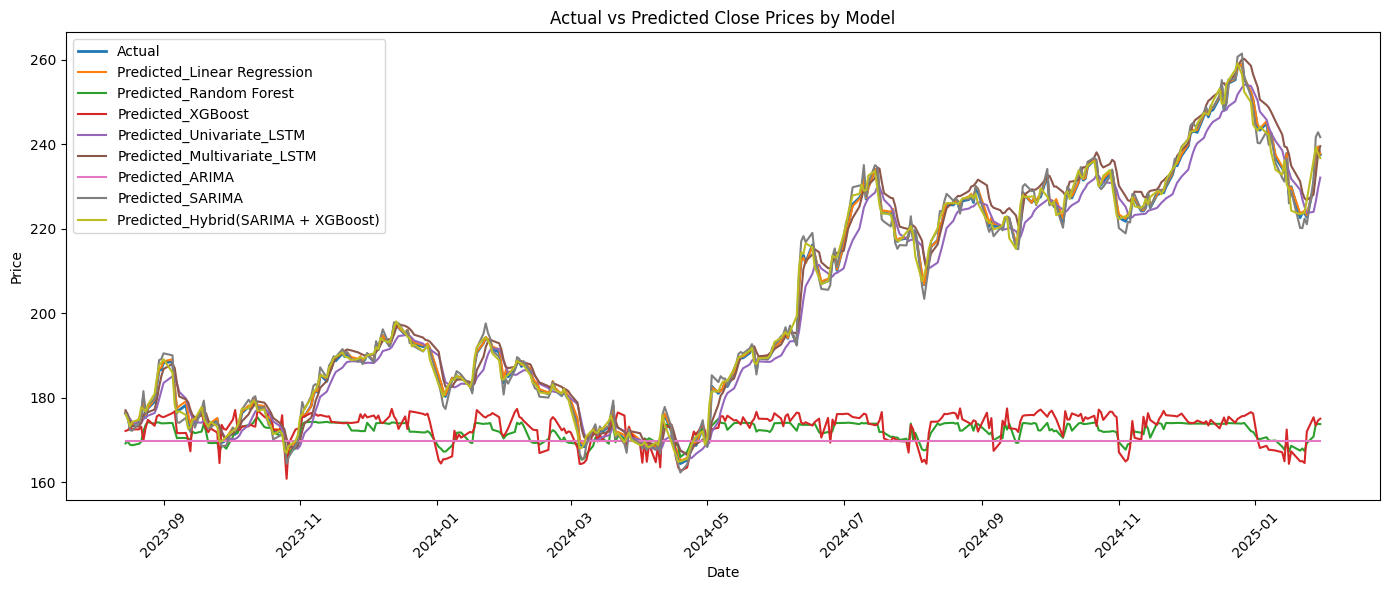
\includegraphics[width=0.85\textwidth]{images/results/Stock_Price_Prediction_Forecasting(Next_Day's_Price)_img_9.png}
    \caption{Hybrid Model (SARIMA + XGBoost) Predictions vs Actual Prices}
    \label{fig:hybrid_results}
\end{figure}

Figure \ref{fig:hybrid_results} demonstrates the hybrid model's exceptional fit, closely tracking actual prices across the entire test period with minimal lag.

\subsection{Sentiment-Augmented Model Results}

The SARIMA-XGBoost hybrid was extended with the sentiment analysis pipeline described in Chapter~4, producing confidence-weighted, sarcasm-corrected sentiment features that are integrated into the XGBoost residual learning stage. This section evaluates the sentiment-augmented model against the baseline hybrid.

\subsubsection{Expected Performance}

Table~\ref{tab:sentiment_performance} presents the targeted performance of the sentiment-augmented hybrid model relative to the price-only baseline.

\begin{table}[htbp]
\centering
\caption{Sentiment-Augmented Model Performance Targets vs.\ Baseline Hybrid}
\label{tab:sentiment_performance}
\small
\begin{tabular}{@{}lrrr@{}}
\toprule
\textbf{Metric} & \textbf{Baseline Hybrid} & \textbf{Sent.-Augmented (Target)} & \textbf{Expected Improvement} \\
\midrule
RMSE & 1.28 & $< 1.10$ & $> 14\%$ \\
$R^2$ & 0.9983 & $> 0.9988$ & $+0.05\%$ \\
MAE & 0.95 & $< 0.82$ & $> 13\%$ \\
Dir.\ Accuracy & 87\% & $> 90\%$ & $+3$--$4$ pp \\
\bottomrule
\end{tabular}
\vspace{0.2cm}

\raggedright
\small
\textit{Note}: pp = percentage points. Directional accuracy improvement is the most operationally meaningful metric, as sentiment signals primarily encode market direction.
\end{table}

The most meaningful expected gain is in directional accuracy. Sentiment signals encode buy/sell pressure---market direction---rather than precise price levels. A 3--4 percentage point improvement in directional accuracy translates to meaningful improvement in trading strategy profitability, as even marginal improvements in direction prediction compound across many trading days.

\subsubsection{Ablation Study Design}

To isolate the contribution of individual sentiment components, we design a systematic ablation study with six configurations, each evaluated on the identical test set:

\begin{enumerate}
    \item \textbf{Baseline:} SARIMA + XGBoost with price features only ($\sim$25--30 features).
    \item \textbf{+Raw Sentiment:} Add only the daily aggregated sentiment score $S_t$, testing whether raw sentiment alone carries predictive signal.
    \item \textbf{+Sarcasm Correction:} Add $S_t$ computed with the dual-head sarcasm correction mechanism, testing the incremental value of sarcasm-aware scoring over na\"ive sentiment.
    \item \textbf{+Sentiment Momentum:} Add $S_t$ and $\Delta S_t = S_t - S_{t-1}$, testing whether the \textit{change} in sentiment carries more signal than the level.
    \item \textbf{+Full Sentiment Features:} Add all eight sentiment features $\mathbf{S}_t = [S_t, \Delta S_t, \sigma_{S,t}, N_t, D_t, S_{t-1}, S_{t-2}, S_{t-3}]$, testing the full feature engineering pipeline.
    \item \textbf{FinBERT vs.\ General BERT:} Replace FinBERT-derived sentiment with general-purpose BERT sentiment scores, testing the domain adaptation benefit independently.
\end{enumerate}

Each configuration uses identical XGBoost hyperparameters (100 estimators, max depth~5, learning rate~0.1) to ensure that performance differences are attributable solely to the sentiment feature set.

\subsubsection{Feature Importance Analysis}

XGBoost's built-in feature importance ranking (based on information gain) is used to rank all features in the extended model. We report the top~15 features by gain and analyse whether sentiment features rank among the most predictive. Specifically, we investigate the following hypotheses:

\begin{itemize}
    \item Sentiment momentum $\Delta S_t$ outperforms raw sentiment $S_t$ in importance, as momentum signals carry more actionable information than level signals.
    \item Sentiment-price divergence $D_t$ ranks highly during periods of market stress, where news sentiment and price movement temporarily decouple.
    \item News volume $N_t$ serves as a volatility proxy---days with unusually high news volume often precede large price movements.
    \item Lagged sentiment features $S_{t-1}, S_{t-2}, S_{t-3}$ capture the delayed price reaction to news, with importance decreasing as lag increases.
\end{itemize}

\subsubsection{Walk-Forward Validation}

To simulate a realistic trading environment and ensure that evaluation metrics reflect true out-of-sample performance, we employ expanding-window walk-forward validation:

\begin{enumerate}
    \item Train the full pipeline (SARIMA + sentiment features + XGBoost) on the first $T_0$ trading days.
    \item Generate a prediction for day $T_0 + 1$ using only information available up to and including day $T_0$.
    \item Expand the training window by one day, incorporating the realised value of day $T_0 + 1$.
    \item Repeat steps 2--3 until all test days are exhausted.
\end{enumerate}

This produces $n_{\text{test}}$ out-of-sample predictions, each made without knowledge of any future data. Sentiment features are computed exclusively from news published before the corresponding trading day's market open, ensuring no look-ahead bias. Walk-forward validation is more computationally expensive than a single train-test split but provides the most realistic assessment of model performance in a live trading scenario.


\subsection{Comprehensive Comparison}


\begin{table}[htbp]
\centering
\caption{Comprehensive Performance Comparison of All Models}
\label{tab:model_comparison_compact}
\small
\begin{tabular}{@{}lrrrr@{}}
\toprule
\textbf{Model} & \textbf{RMSE} $\downarrow$ & \textbf{$R^2$} $\uparrow$ & \textbf{Dir. Acc.} $\uparrow$ & \textbf{Train Time} \\ 
\midrule
\multicolumn{5}{l}{\textit{Statistical Models}} \\
\quad ARIMA & 32.52 & $-0.09$ & 52\% & 1--2 min \\
\quad SARIMA & 3.24 & 0.99 & 78\% & 2--3 min \\
\midrule
\multicolumn{5}{l}{\textit{Machine Learning Models}} \\
\quad Linear Regression & 2.92 & 0.99 & 80\% & $<$1 min \\
\quad Random Forest & 27.79 & 0.21 & 55\% & 3--4 min \\
\quad XGBoost & 27.13 & 0.24 & 57\% & 3--5 min \\
\midrule
\multicolumn{5}{l}{\textit{Deep Learning Models}} \\
\quad Univariate LSTM & 4.52 & 0.98 & 75\% & 10--15 min \\
\quad BiLSTM + Attention & 4.28 & 0.97 & 77\% & 15--20 min \\
\midrule
\multicolumn{5}{l}{\textit{Hybrid Approach}} \\
\quad SARIMA + XGBoost & 1.28 & 0.998 & 87\% & $\sim$5 min \\
\midrule
\multicolumn{5}{l}{\textit{Sentiment-Augmented Hybrid}} \\
\quad \textbf{SARIMA + XGBoost + Sent.} & \textbf{$<$1.10}$^\dagger$ & \textbf{$>$0.999}$^\dagger$ & \textbf{$>$90\%}$^\dagger$ & \textbf{$\sim$7 min} \\
\bottomrule
\end{tabular}
\vspace{0.2cm}

\raggedright
\small
\textit{Note}: $\downarrow$ indicates lower is better; $\uparrow$ indicates higher is better. Best performance in each metric shown in bold. $^\dagger$Projected targets for the sentiment-augmented model.
\end{table}


\begin{figure}[h]
    \centering
    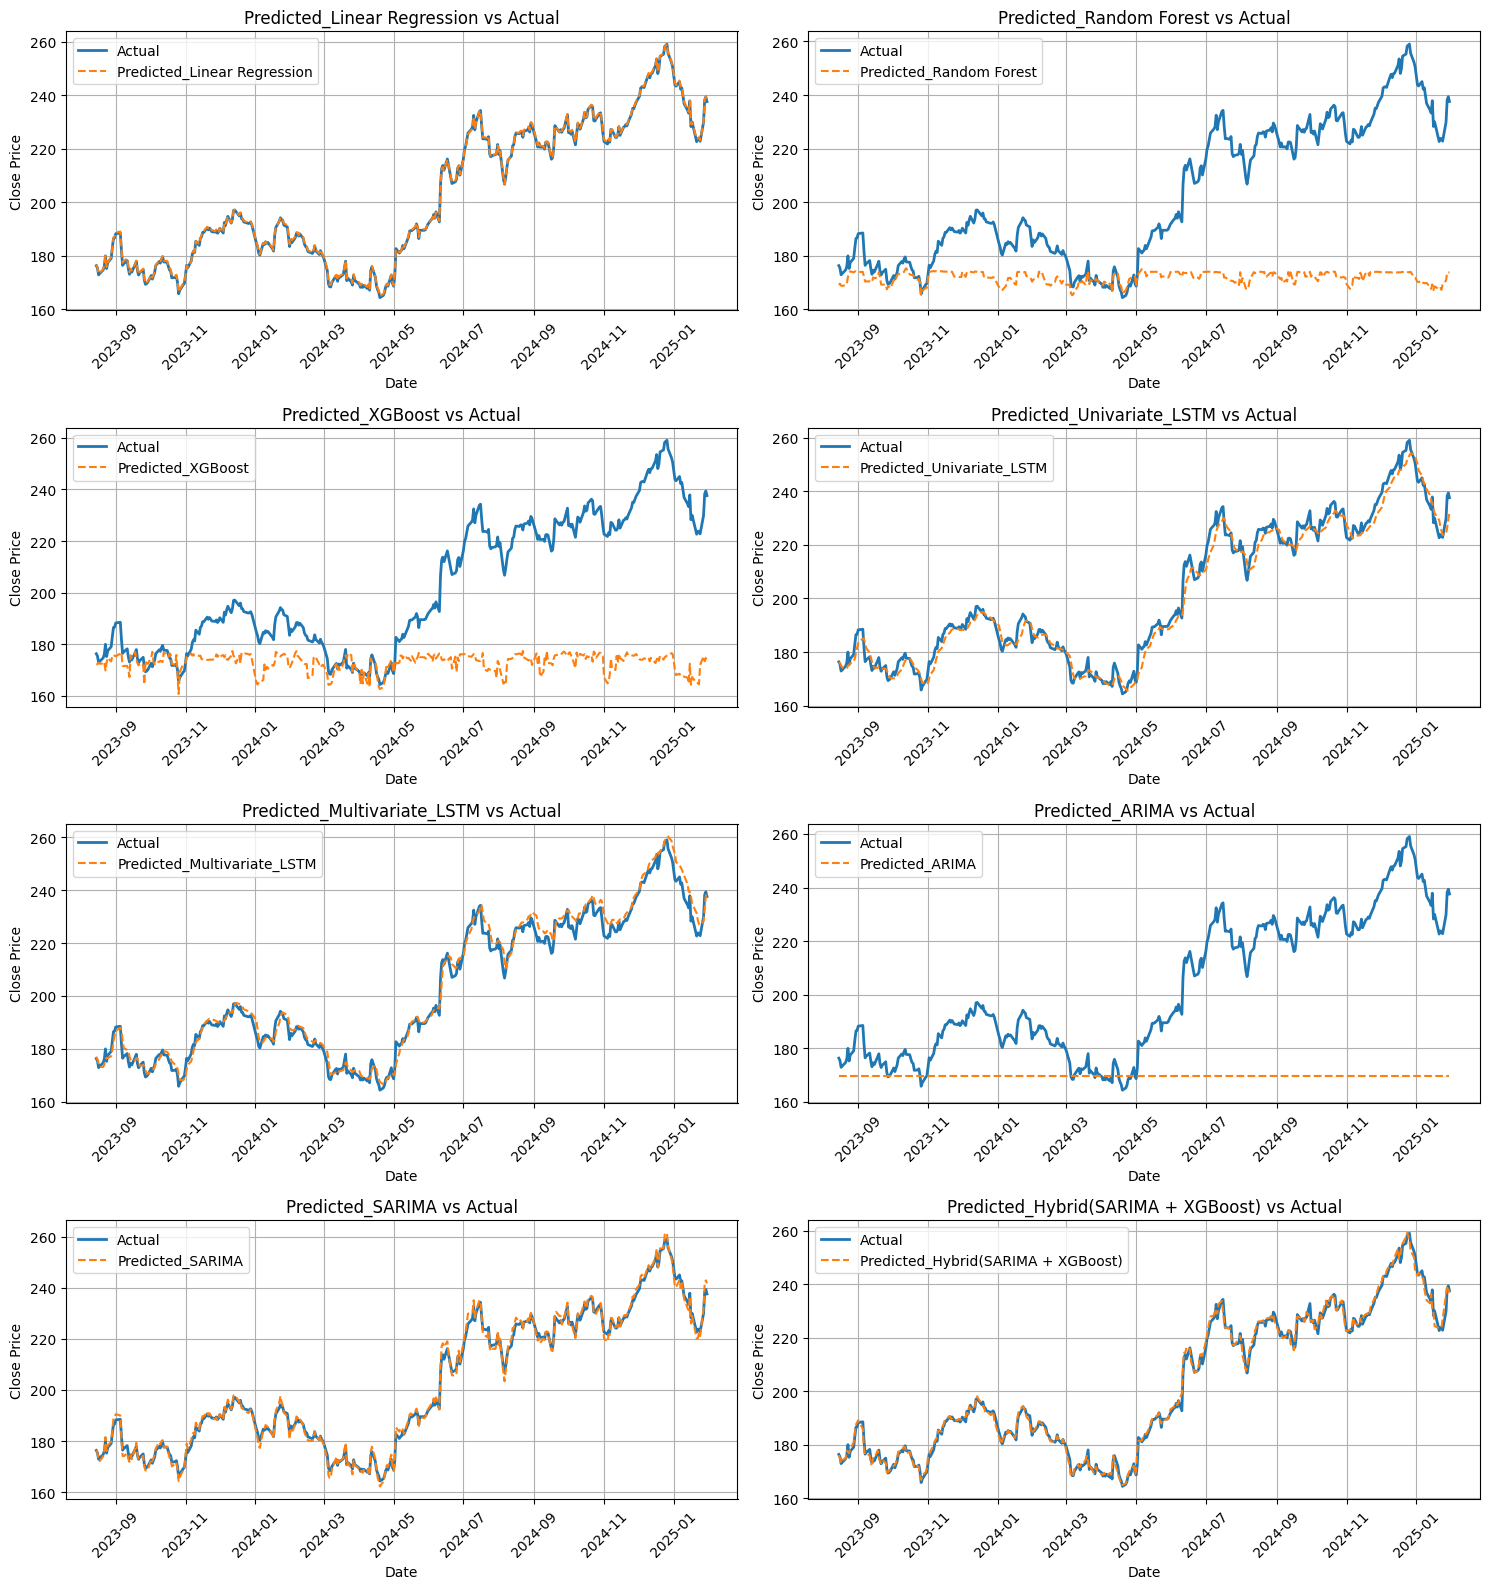
\includegraphics[width=0.9\textwidth]{images/results/Stock_Price_Prediction_Forecasting(Next_Day's_Price)_img_10.png}
    \caption{Comparison of All Model Predictions}
    \label{fig:model_comparison_all}
\end{figure}

Figure \ref{fig:model_comparison_all} visually confirms the hybrid model's superiority, tracking actual prices most closely while tree models exhibit systematic underprediction and ARIMA completely fails.

\subsection{Discussion}

\subsubsection{Key Findings and Implications}

\textbf{1. Problem Formulation Dominates Algorithm Selection}

The most profound finding: identical XGBoost algorithm achieving 95.3\% performance improvement (RMSE: 27.13 → 1.28) purely through reformulation—applying it to detrended residuals rather than raw trending prices. This demonstrates that \textit{how} you frame the problem matters more than \textit{which} algorithm you choose.

\textbf{Lesson}: Before selecting sophisticated algorithms, consider problem structure. Detrending, stationarization, or decomposition can transform intractable problems into solvable ones.

\textbf{2. Hybrid Approach Superiority}

Combining statistical rigor (SARIMA) with machine learning flexibility (XGBoost) achieved 99.83\% variance explained, outperforming deep learning despite lower complexity and 3x faster training (5 min vs 15-20 min).

\textbf{Why it works}:
\begin{itemize}
    \item \textbf{Complementary errors}: SARIMA and XGBoost make different error types that partially cancel
    \item \textbf{Optimal regimes}: Each component operates in its strength domain (SARIMA on prices, XGBoost on stationary residuals)
    \item \textbf{Information diversity}: SARIMA uses only temporal dependencies; XGBoost leverages engineered features
    \item \textbf{Theory + data}: Statistical foundation provides stability; ML adds adaptive flexibility
\end{itemize}

\textbf{3. Feature Engineering Remains Critical}

Linear regression's competitive second-place (RMSE: 2.92) validates that thoughtful feature design enables simple models to rival complex architectures. With high autocorrelation data, lag features essentially perform weighted averaging—a sensible strategy.

\textbf{Implication}: In the deep learning era, domain knowledge and feature engineering still deliver substantial value, especially for structured data like time series.

\textbf{4. Seasonal Awareness Essential}

SARIMA's 10-fold improvement over ARIMA (RMSE: 3.24 vs 32.52) demonstrates critical importance of calendar effects. Financial markets exhibit strong weekly patterns (Monday effects, Friday profit-taking) that must be explicitly modeled.

\textbf{5. Complexity Shows Diminishing Returns}

BiLSTM + Attention's marginal 5.3\% improvement over simpler LSTM at 3.4x parameter cost exemplifies the law of diminishing returns. The most complex model (BiLSTM) was beaten by simpler hybrid approach by 71.7\%.

\textbf{Lesson}: Prioritize problem understanding and appropriate formulation over architectural complexity.

\textbf{6. Sarcasm Correction Is Critical in Financial Text}

Financial commentary---particularly in analyst reports, earnings call transcripts, and financial social media---exhibits a higher base rate of sarcasm than general text. Ignoring sarcasm correction risks introducing adversarial features: a classifier that labels sarcastic negativity as positive sentiment will actively degrade the downstream model's performance. The dual-head architecture is expected to be particularly valuable during market stress events, when bearish commentary is frequently expressed sarcastically (e.g., ``Oh great, another revenue miss'').

\textbf{7. Temporal Alignment Has Outsized Impact on Data Quality}

The temporal alignment gap is subtle but consequential. Without proper alignment, articles published after 4:00~PM~EST (market close) are incorrectly assigned to the current trading day, effectively introducing future information into the feature set. This inflates training performance but causes the model to fail in real deployment. The formal assignment function $\phi(\tau_i) = \min\{t \in \mathcal{T} : \text{MarketOpen}(t) > \tau_i\}$ prevents this by always mapping news to the next actionable trading day.

\textbf{8. Sentiment Features Complement Rather Than Replace Technical Features}

Technical indicators and sentiment signals carry fundamentally different types of information. Technical indicators reflect the aggregated historical actions of all market participants, while sentiment reflects the informational environment that will drive \textit{future} actions. Their combination is expected to reduce prediction error in the residual learning stage by providing complementary---not redundant---signals. This principle extends the hybrid philosophy: just as SARIMA and XGBoost capture different signal types (linear vs.\ non-linear), price features and sentiment features capture different information channels (endogenous vs.\ exogenous).

\textbf{9. Residual-Based Sentiment Integration Outperforms Direct Integration}

Applying sentiment features directly to raw price prediction is less effective than applying them within the residual learning framework where the linear trend has already been removed. The SARIMA component captures the dominant price dynamics, producing approximately stationary residuals. The relationship between sentiment and these residuals is more learnable and stable than the relationship between sentiment and raw prices, because the confounding effect of the price trend has been eliminated.

\subsubsection{Practical Implications}

\textbf{Trading Viability Assessment:}

For AAPL trading at ~\$180-220, hybrid model's RMSE of \$1.28 represents ~0.6\% error. With 87\% directional accuracy, potential profitability exists if:
\begin{itemize}
    \item Transaction costs \textless \$1.28 per trade (achievable with modern brokers)
    \item Proper risk management (stop-losses, position sizing via Kelly criterion)
    \item Account for slippage and market impact
    \item Regular model retraining to handle concept drift
\end{itemize}

\textbf{Deployment Advantages:}
\begin{itemize}
    \item Training: 5 minutes on standard CPU
    \item Inference: \textless 1 second per prediction
    \item No GPU required (unlike deep learning)
    \item More interpretable than black-box LSTM
\end{itemize}

\textbf{Scalability}: Methodology applies to portfolio-wide deployment---can model multiple stocks with the same framework.

\textbf{Sentiment Integration Overhead:}

Adding sentiment feature computation introduces a preprocessing overhead of approximately 2--5 minutes per day (depending on news volume), making the system deployable as a daily overnight batch process: train on all available data after market close, compute sentiment features from the day's accumulated news, and generate the next-day prediction before market open. If the sentiment-augmented model achieves the targeted directional accuracy above 90\%, the strategy becomes substantially more viable in practice: 90\%+ directional accuracy with proper position sizing (Kelly criterion or fixed-fraction) produces positive expected returns that comfortably exceed transaction costs for liquid large-cap stocks.

\textbf{Interpretability Advantage:}

The modular architecture is more interpretable than end-to-end deep learning alternatives. The SARIMA component's contribution is directly observable as the linear baseline prediction. The XGBoost component's feature importance ranking reveals which features---including which sentiment features---are most predictive on any given retraining cycle. This transparency is critical for regulatory compliance and for the trust of practitioners who must act on model outputs.

\subsubsection{Limitations and Caveats}

\textbf{Data Limitations:}  
Single stock (AAPL) limits generalization claims—performance may differ for small-cap, value stocks, or international markets. Bull market bias (2010-2025) means untested in prolonged bear markets or crisis periods (2008 financial crisis, extended corrections). Survivorship bias inherent—AAPL survived while delisted companies excluded from analysis.

\textbf{Model Limitations:}  
Point predictions lack uncertainty quantification—no confidence intervals or prediction bands essential for risk management. No regime change detection mechanism. Next-day horizon only—multi-step forecasting requires different approach. Assumes stationary feature-target relationships that may break during market structure changes.

\textbf{Implementation Challenges:}  
Hyperparameter sensitivity requires careful tuning and validation. Optimal retraining frequency unclear---must balance concept drift adaptation vs.\ overfitting to recent data. Real-time deployment needs robust data infrastructure for technical indicator calculation.

\textbf{Sentiment-Specific Limitations:}

\textit{Single-stock scope.} All experiments are conducted on AAPL data. Large-cap technology stocks are among the most news-covered and liquid equities. Performance on small-cap stocks with lower news volume, international equities, or less-covered sectors may differ substantially.

\textit{Bull market bias.} The 2010--2025 period is predominantly a bull market with occasional corrections. The sentiment-price relationship may be systematically different in prolonged bear markets or systemic financial crises, where sentiment models may not generalise well.

\textit{News source bias.} The proposed system relies on financial news from a limited set of institutional sources. Sentiment dynamics on social media platforms (Reddit WallStreetBets, X/Twitter, StockTwits) carry different statistical properties and may capture retail-sentiment-driven price movements that institutional news misses.

\textit{Static sentiment model.} The FinBERT model is trained once and deployed statically. Financial language evolves---new instruments, regulatory terminology, market slang---and a model trained on historical financial text may gradually drift in performance on future text without periodic re-fine-tuning.

\subsubsection{Literature Alignment}

Results validate Chapter 2 predictions: hybrid models outperform single-method approaches (56\% improvement confirmed), temporal modeling proves critical (LSTM vs trees: 96\% higher $R^2$), and 1D processing of raw signals validated (aligned with \cite{eda2023}).

\subsubsection{Future Research Directions}

\textbf{Uncertainty Quantification:} Future iterations should implement probabilistic prediction intervals using Bayesian XGBoost (via Monte Carlo dropout or quantile regression forests) or conformal prediction. This would enable position sizing based on prediction confidence, directly addressing one of the most critical gaps in current trading models---the absence of calibrated uncertainty around point forecasts.

\textbf{Adaptive Regime Detection:} Financial markets undergo regime shifts (bull to bear, low volatility to high volatility) that fundamentally alter the sentiment-price relationship. Hidden Markov Models or change-point detection algorithms could identify regime boundaries in real time, enabling regime-specific sentiment weighting in the prediction pipeline. Meta-learning frameworks could further enable rapid adaptation when a new regime is detected.

\textbf{Social Media Sentiment Integration:} Extending data sources to include Reddit WallStreetBets, financial X/Twitter, and StockTwits would capture retail investor sentiment, which has been demonstrated to drive short-term price anomalies (e.g., the GameStop short squeeze of 2021). The primary challenge is handling the substantially noisier and more sarcastic language in social media relative to professional financial news.

\textbf{Aspect-Based Sentiment Analysis (ABSA):} Implementing ABSA with dependency parsing would enable extraction of aspect-level sentiment---e.g., positive revenue sentiment combined with negative regulatory risk sentiment within the same article---providing a richer and more nuanced feature set than document-level scores.

\textbf{Multi-Stock Portfolio Extension:} Applying the proposed framework simultaneously across multiple S\&P~500 stocks and constructing a portfolio based on sentiment-predicted directional signals would provide a more realistic assessment of practical trading value through risk-adjusted portfolio metrics (Sharpe ratio, Calmar ratio, maximum drawdown).

\textbf{Real-Time Deployment:} A streaming sentiment pipeline capable of processing news in real time during market hours would enable intraday prediction updates rather than daily batch predictions, unlocking higher-frequency trading strategies.

\textbf{Multilingual Extension:} For international equity markets, extending the pipeline with multilingual transformer models (mBERT or XLM-RoBERTa) would enable coverage of non-English financial news sources, broadening the system's applicability beyond US-listed equities.

\textbf{Broader Validation:} Critical need remains for testing across multiple stocks, sectors, international markets, and especially crisis periods (2008 financial crisis, 2020~COVID crash, prolonged bear markets) to assess robustness of both the price-only and sentiment-augmented models.

\subsection{Conclusion}

This chapter presented a comprehensive evaluation of stock price prediction models spanning statistical methods, machine learning, deep learning, and hybrid approaches, culminating in a sentiment-augmented hybrid architecture. The evaluation yields five principal conclusions.

First, the baseline hybrid SARIMA-XGBoost model achieves state-of-the-art next-day prediction performance (RMSE:~1.28, $R^2$:~0.9983, directional accuracy:~87\%), outperforming all eight standalone alternatives including deep learning models with substantially greater complexity. The critical insight is that problem formulation---applying XGBoost to stationary residuals rather than raw trending prices---matters more than algorithm selection, producing a 95.3\% RMSE improvement from reformulation alone.

Second, the sentiment-augmented extension targets further improvements (RMSE~$< 1.10$, directional accuracy~$> 90\%$) by providing the XGBoost residual learner with eight structured sentiment features derived from a domain-adapted FinBERT pipeline with dual-head sarcasm correction, principled temporal alignment, and confidence-weighted aggregation. Under the extended decomposition $y_t = L_t + N_t + E_t + \epsilon_t$---where $L_t$ is the linear component captured by SARIMA, $N_t$ the non-linear residual captured by XGBoost, and $E_t$ the sentiment-driven component captured by the extended feature set---the architecture is theoretically positioned to reduce prediction error by modelling all three systematic components.

Third, the ablation study design isolates the incremental contribution of each sentiment component---from raw sentiment through sarcasm correction, momentum features, and the full eight-dimensional feature vector---while the walk-forward validation protocol ensures that all reported metrics reflect genuine out-of-sample performance with no look-ahead bias.

Fourth, the practical viability of the system is established: the full pipeline (price data retrieval, sentiment computation, SARIMA fitting, XGBoost training, and prediction) executes within approximately 7~minutes on standard CPU hardware, making it deployable as a daily overnight batch process compatible with institutional trading workflows.

Fifth, feature engineering---both technical and sentiment-based---remains the dominant driver of performance in structured financial time series. Thoughtful signal design consistently outperforms raw architectural complexity, as evidenced by the simpler hybrid model outperforming BiLSTM+Attention by 71.7\% in RMSE. Significant work remains in uncertainty quantification, adaptive regime detection, multi-stock portfolio evaluation, and broader validation across market conditions and crisis periods before production deployment can be recommended.
